\newpage

\section{Measuring Area}

\begin{teachingnote}
Supplies: Bring extra copies of the sheet (for restarting after mistakes).  Bring extra rulers. 

Nominally, this activity is about verifying that the triangle area formula gives the same result no matter which
side is chosen as the ``base.''  But the activity also allows some other challenges to come to the surface:  
\begin{itemize}
\item Some students do not realize that sometimes the line containing the base must be 
extended to allow the height to be drawn. 
\item Some students have trouble drawing a perpendicular line when the given line is neither vertical nor 
horizontal on the page.  Conceptually, this is an opportunity to highlight the definition of right angle:  An angle formed when two lines intersect so that adjacent angles are congruent.  Mechanically, students can take advantage of the fact that the tick marks on 
a ruler are perpendicular to the edge of the ruler.  
\item Some students have trouble measuring fractions of inches, sometimes thinking that the tick marks are tenths.  
\end{itemize}
\end{teachingnote}

\begin{prob}
Three congruent triangles are shown below.   
\begin{enumerate}
\item For each triangle, choose a base and use a ruler to draw carefully the corresponding height to that base.  (Choose bases of different lengths.)  Remember:  A \emph{height} is measured on a line that is perpendicular to a base and containing the opposite vertex. 
\item Measure the heights and bases accurately, and compute the area of each triangle.  
\item What do your results demonstrate about the formula for the area of a triangle?  
\end{enumerate}

\vfill
\begin{fullwidth}
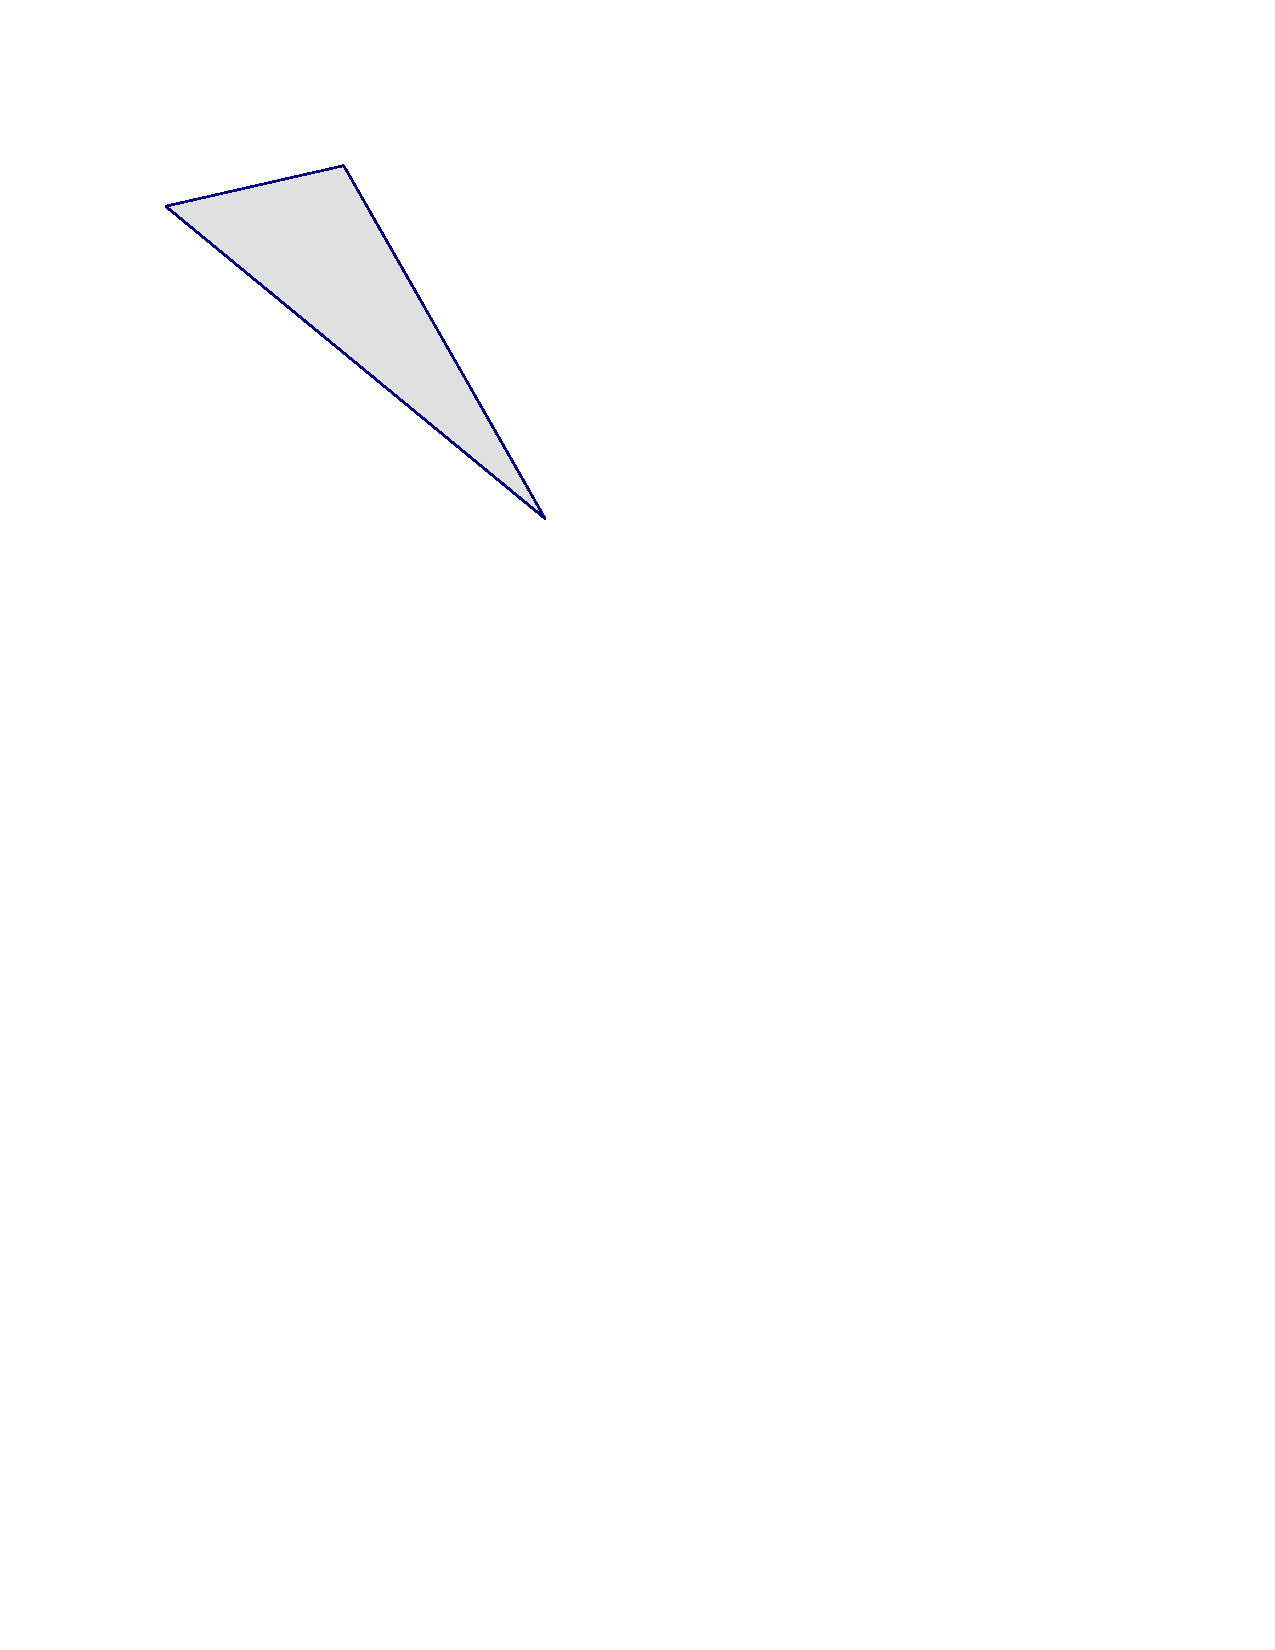
\includegraphics{../graphics/triangle.pdf}
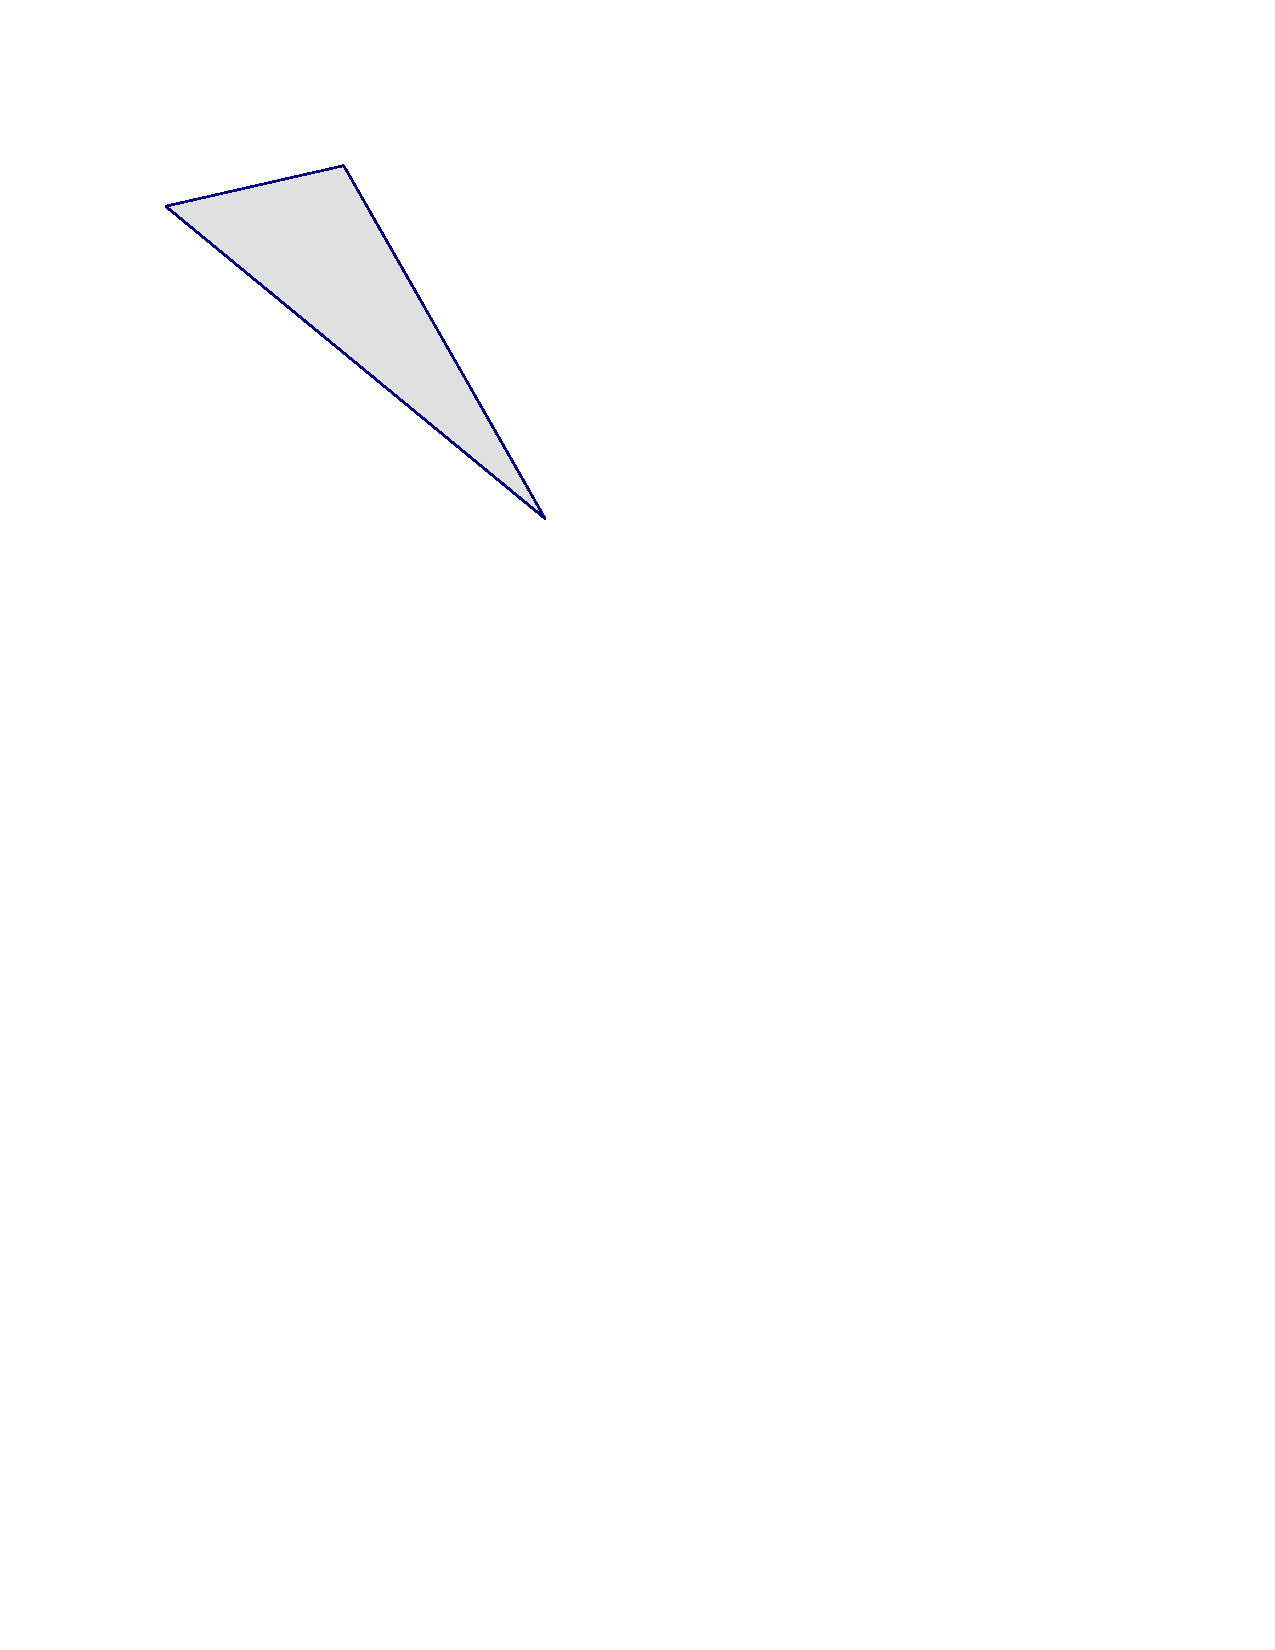
\includegraphics{../graphics/triangle.pdf}
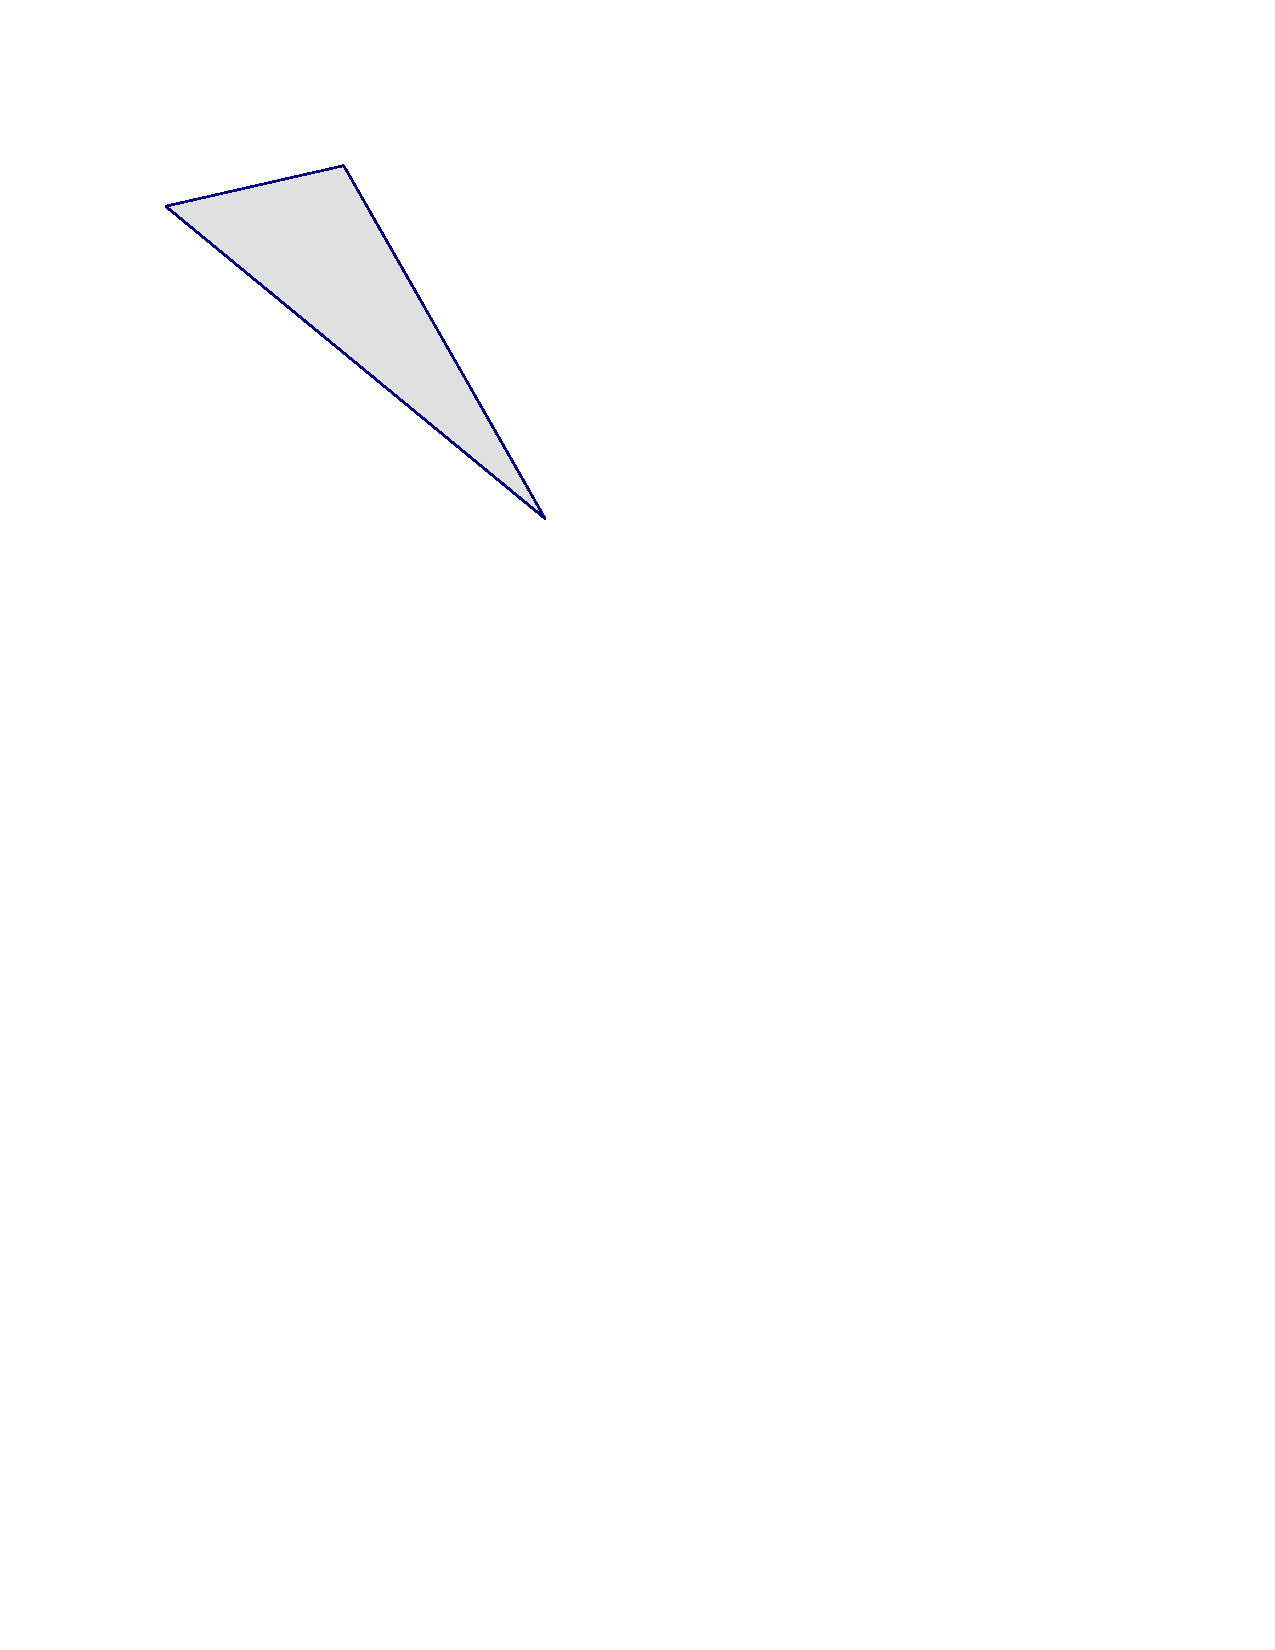
\includegraphics{../graphics/triangle.pdf}
\end{fullwidth}

\end{prob}
\vfill
